% Appendix A

\chapter{Implementing Dynamic Energy Map in
  ArcGIS} % Main appendix title

\label{AppendixC} % For referencing this appendix elsewhere, use \ref{AppendixA}

\lhead{Appendix C. \emph{Dynamic Energy Map in ArcGIS}} % This is for the header on each page - perhaps a shortened title
\section{Introduction}
This section records the process of implementing a dynamic energy map
in ArcGIS. The computer used in this implementation is a Dell
Precision T1600 Quad Core Intel Xeon, 3.10GHz machine with 16GB RAM in
CMU Baker 140C cluster. The GIS software used is ArcScene
10.2~\cite{arcScene2015}.

The common procedure is 1) to export CityEngine models as either gdb
file or as collada files and import the model to ArcScene 2)
preprocess the energy profile and write it to a csv file containing
hourly energy consumption for all building types in the
community. 3) join the table to the 3D features 4) enable time in the
joint layer and 5) configurate the setting of the animation and play
the animation in ArcGIS. Each step will be explained in more detail in
the following session.
\section{Explaining Each Steps}
\begin{enumerate}[1)]
\item Exporting CityEngine model. 

  The exported format could be a) gdb file that contains the object
  attributes of building lots or b) collada file that only contains
  the model geometry. Method a), the advantage is its potential to
  pass attribute information from CityEngine to ArcGIS. Method b)
  requires a small script so that each building geometry could be
  exported as one collada file.

\item Produce a file containing the energy profile of all buildings in
  the community model into a csv file with one date-time column
  containing the time information and several energy profile
  information. 

  The number of rows equals to $n \times 8760$ where $n$ is the unique
  building types (if two building has different energy demand
  behavior, they are considered to have different types).
  \fref{fig:importCSV} shows the file used in this implementation
  example. The first column contains the time information. The format
  of the time column is crutial because it will be converted to a
  ``date'' type in later steps. This conversion requires the input csv
  file have one of its suggested date-time format. The format addopted
  in this example is ``yyyy/mm/dd one space HH:MM:SS''. The range of
  the ``HH'' should be 0 to 23 (not 1 to 24). The second column is the
  hourly gas heating energy demand in kBtu and the third column is the
  hourly cooling energy demand in kBtu. The forth column contains a
  short integer corresponding to the building type this row of energy
  file represents.

\begin{figure}[h!]
  \centering
  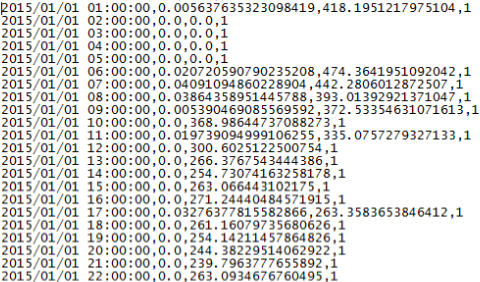
\includegraphics[width=0.7\linewidth]{importCSV.png}
  \caption[Imported CSV]{A screenshot of the energy profile in csv
    format to be imported to ArcScene}
  \label{fig:importCSV}
\end{figure}

\item After importing the table to the working file geodatabase, one
  should use the ``convert time field'' to covert the time column in
  the imported csv table to type ``date''.

\item Create the centroid for each building geometry footprint As is
  mentioned in \sref{sec:aggregateTime}, aggregating the energy data
  of the whole year to the 3D building geometry is not achievable with
  the machine used in this example. So here the authors chose to
  aggregate the energy data into a simplefiled geometry representation
  of the buildings in the community model: the centroid of each
  building. The steps of aggregating energy data to 3D building
  features is the same as the steps of aggregating energy data to
  building centroid by just changing the layer to which the data is
  joined. An animated version of such aggregation can be accessed
  \href{http://www.armechxyj.com/energy-mapping.html#arcgisAnime}{at
    this link}. \fref{fig:animeArcGIS} shows a screenshot of the
  ArcScene Dynamic Map showing the hourly gas heating energy demand. 

\begin{figure}[h!]
  \centering
  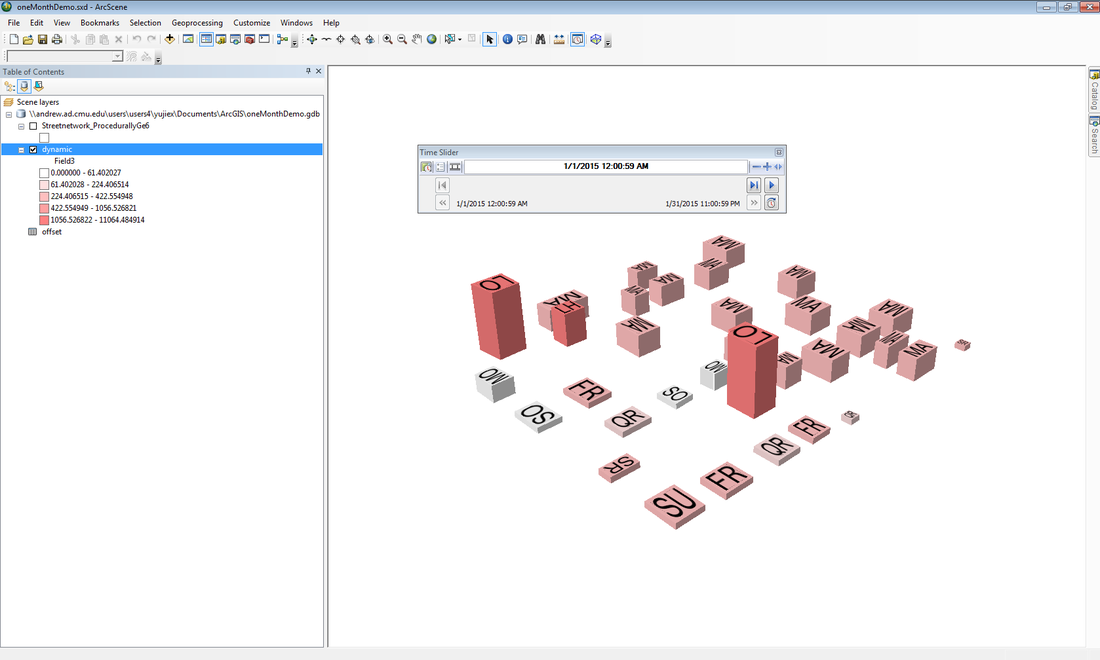
\includegraphics[width=0.7\linewidth]{animeArcGIS.png}
  \caption[3D Dynamic Heat Map in ArcGIS]{A screen shot of a dynamic
    energy map in ArcGIS, the legend on the left shows the hourly gas
    heating energy demand}
  \label{fig:animeArcGIS}
\end{figure}

The way to create building centroid is to first add two extra field in
attribute table of the imported building lot feature class
(``streetnetworkPaste'') and use ``Calculate Geometry'' to retrieve
the x, y coordinate of the centroid for each building lot
(\fref{fig:cenTable}).
\begin{figure}[h!]
  \centering
  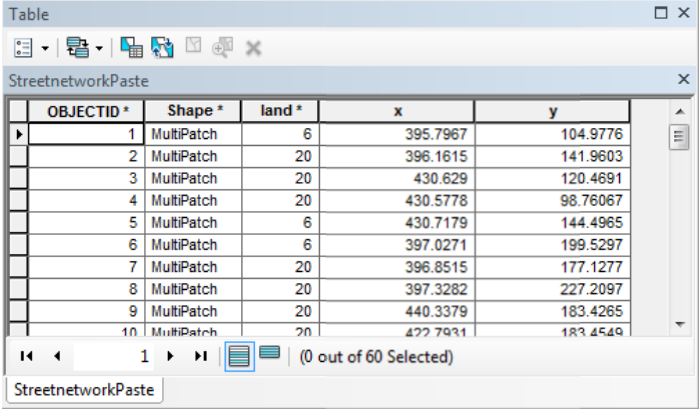
\includegraphics[width=0.7\linewidth]{cenTable.png}
  \caption[Calculated Centroid]{Calculated Centroid}
  \label{fig:cenTable}
\end{figure}

Then export the table to the working gdb and use ``make x y event
layer'' tool to create a point feature (``cen'')
(\fref{fig:cenFeature})
\begin{figure}[h!]
  \centering
  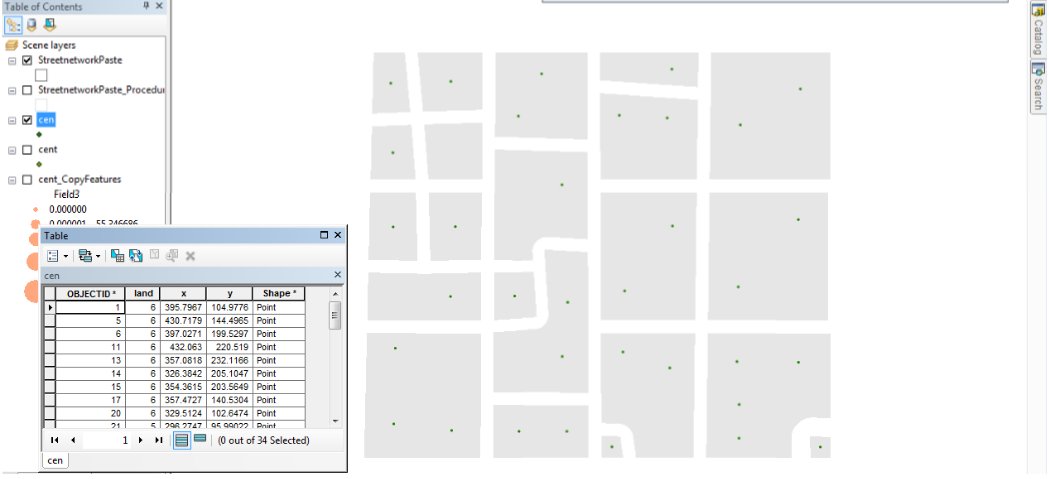
\includegraphics[width=0.7\linewidth]{cenFeature.png}
  \caption[Created Centroid Feature]{The centroid feature is created
    with the x y table}
  \label{fig:cenFeature}
\end{figure}

\item Import the centroid layer (``cen'') to the working gdb. 

  This step important, because in the documentation about ``join'',
  ``When you create a join in such a case (one-to-many or many-to-
  many), there are differences between how tools and other
  layer-specific settings work depending on the data source. If you
  are using geodatabase data to create the join, all matching records
  are returned. If you are using nondatabase data, like shapefiles or
  dBASE tables, to create the join, only the first matching record is
  returned.''~\cite{GISjoin2014} If we do not import it to gdb file,
  the record that retains are only one row for each building type,
  which is not desirable for the current situation. In order to retain
  all 8760 matching records for each building type, importing the
  feature class and table to gdb is crutial.

\item Add ``Attribute Index'' to the feature class to the centroid
  layer to be joint.
  
  The index acted as search keys in the database. Adding index makes
  searching of matching data faster. In our current case, the search
  key should be ``landuse''
  
\item Use ``Add join'' tool to join the centroid and the energy
  profile table with ``landuse'' as a matching field

  After the add join, when opening the ``attribute table'' of the
  centroid layer, one could not see all the matching records, but one
  can still have a feeling they are retained because the model will
  become very slow. 

\item Use ``copy features'' tool to copy the joint centroid layer to a
  new layer, then all the matching features are visible
  (``cent\_CopyFeatures'') (\fref{fig:aggTable})
  
\begin{figure}[h!]
  \centering
  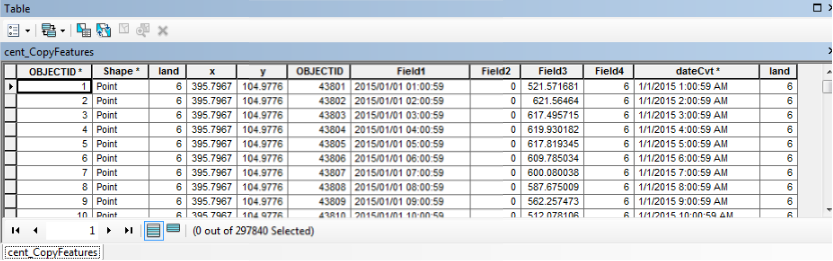
\includegraphics[width=0.7\linewidth]{aggTable.png}
  \caption[Table with Time]{The copied table retains all 8760 building
    energy information of the buildings in the community model, there
    are in total $8760 \times 34 = 297840$ rows of data entries in the
    table because there are 34 buildings in the community model}
  \label{fig:aggTable}
\end{figure}

An alternative of ``add join $+$ copy features'' of creating a feature
class that aggregates the spatial geometry and the temporal energy
demand is through the tool ``make query table'', detailed explanation
of this tool is explained in \cite{queryTable2012}.

\item Change the symbol to be graduated symbols, with ``Quantile
  method'' as the current classification method to ensure a larger
  variation in symbol changes for demonstration purpose. The ``sample
  size'' of classification breakpoint should be reset so that it is at
  not smaller than the total number of data points (number of rows in
  the final attribute table) 
  
\item Enable ``time'' on the final layer (``cent\_CopyFeatures'') with
  aggregated time, energy data and geometry.

\item Add the time-column as an Attribute Index to the final layer and
  one can configure the animation play back to play the animated
  maps. 

  Although it is surprising that this step is not done automatically,
  this step is crucial. If one does not add it, one may find the
  render of the image in the slider very slow even though one set the
  ``playback'' to fast.
\end{enumerate}

\subsection{Final Output}
In order to make the symbol more visible, an orthogonal top view was
chosen as the map view port. The building geometry layer is for
providing a spatial context, thus a transparent filling was applied to
this layer. \fref{fig:centroidMap} shows a screen shot of the animated
map interface inside stand-alone ArcScene. The exported animation
version could be found
\href{http://www.armechxyj.com/energy-mapping.html#slowAnime}{through
  this link}.

\begin{figure}[h!]
  \centering
  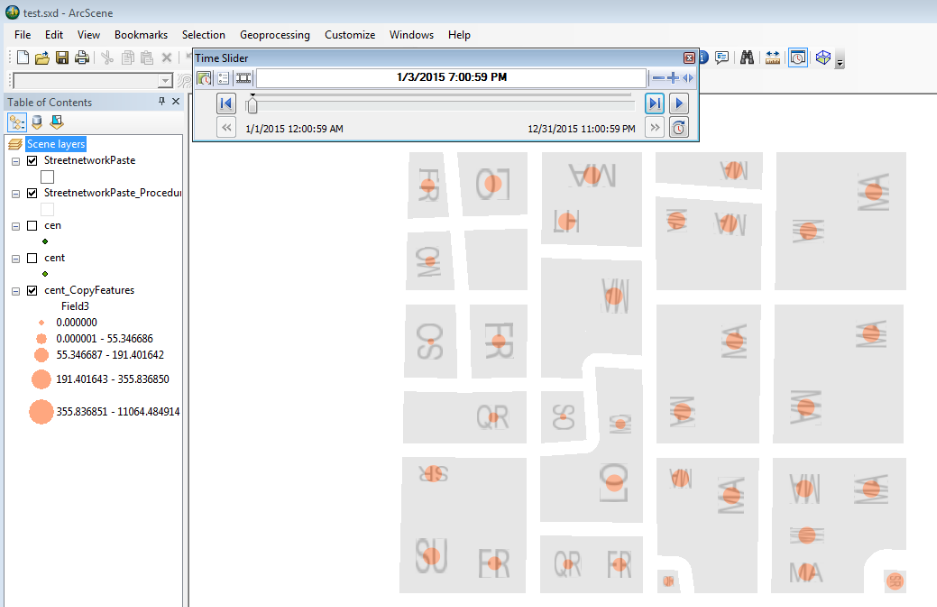
\includegraphics[width=0.7\linewidth]{centroidMap.png}
  \caption[Dynamic Map in ArcScene with Building Centroid]{A
    screenshot of the dynamic map interface in ArcScene 10.2, the
    hourly heating energy are represented as a graduated-sized point
    symbol with larger size for larger demand}
  \label{fig:centroidMap}
\end{figure}

One issue regarding using ArcScene as the generator of images for 3D
visualization is that the ``DataFrame'' module in image exporting does
not work for ArcScene, this means we cannot export 3D map image
sequences for later post processing and display. This acts as another
drawback that disables us from using ArcGIS in producing map images
for implementing a dynamic energy map.